\documentclass[12pt,letterpaper]{article}
\usepackage[utf8]{inputenc}
\usepackage[spanish]{babel}
\usepackage{graphicx}
\usepackage[left=2cm,right=2cm,top=2cm,bottom=2cm]{geometry}
\usepackage{graphicx} % figuras
% \usepackage{subfigure} % subfiguras
\usepackage{float} % para usar [H]
\usepackage{amsmath}
%\usepackage{txfonts}
\usepackage{stackrel} 
\usepackage{multirow}
\usepackage{enumerate} % enumerados
\renewcommand{\labelitemi}{$-$}
\renewcommand{\labelitemii}{$\cdot$}
% \author{}
% \title{Caratula}
\begin{document}

% Fancy Header and Footer
% \usepackage{fancyhdr}
% \pagestyle{fancy}
% \cfoot{}
% \rfoot{\thepage}
%

% \usepackage[hidelinks]{hyperref} % CREA HYPERVINCULOS EN INDICE

% \author{}
\title{Caratula}

\begin{titlepage}
\begin{center}
\large{UNIVERSIDAD PRIVADA DE TACNA}\\
\vspace*{-0.025in}
\begin{figure}[htb]
\begin{center}

\includegraphics[width=8cm]{./Imagenes/logo}
\end{center}
\end{figure}
\vspace*{0.15in}
INGENIERIA DE SISTEMAS \\

\vspace*{0.5in}
\begin{large}
TITULO:\\
\end{large}

\vspace*{0.1in}
\begin{Large}
\textbf{INFORME DE LABORATORIO N03 -Creando un Reporte Interactivo en Power BI} \\
\end{Large}

\vspace*{0.3in}
\begin{Large}
\textbf{CURSO:} \\
\end{Large}

\vspace*{0.1in}
\begin{large}
INTELIGENCIA DE NEGOCIOS\\
\end{large}

\vspace*{0.3in}
\begin{Large}
\textbf{DOCENTE(ING):} \\
\end{Large}

\vspace*{0.1in}
\begin{large}
 Patrick Cuadros Quiroga\\
\end{large}

\vspace*{0.2in}
\vspace*{0.1in}
\begin{large}

\begin{flushleft}
Alumno: \\
Damian Mamani, David Reynaldo 		\hfill	(2016055194) \\
\end{flushleft}
\end{large}
\end{center}

\end{titlepage}


\tableofcontents % INDICE
\thispagestyle{empty} % INDICE SIN NUMERO
\newpage
\setcounter{page}{1} % REINICIAR CONTADOR DE PAGINAS DESPUES DEL INDICE

\section{Desarrollo } 

\subsection {Crear Relaciones}
\begin{itemize}
 \item 1.Conectando a Power Bi a datos
 Copiar el script Task 1 del archivo Lab Exercise1.sql. y pegar la consulta en Power BI, en el cuadro sentencia SQL.
	\begin{center}
	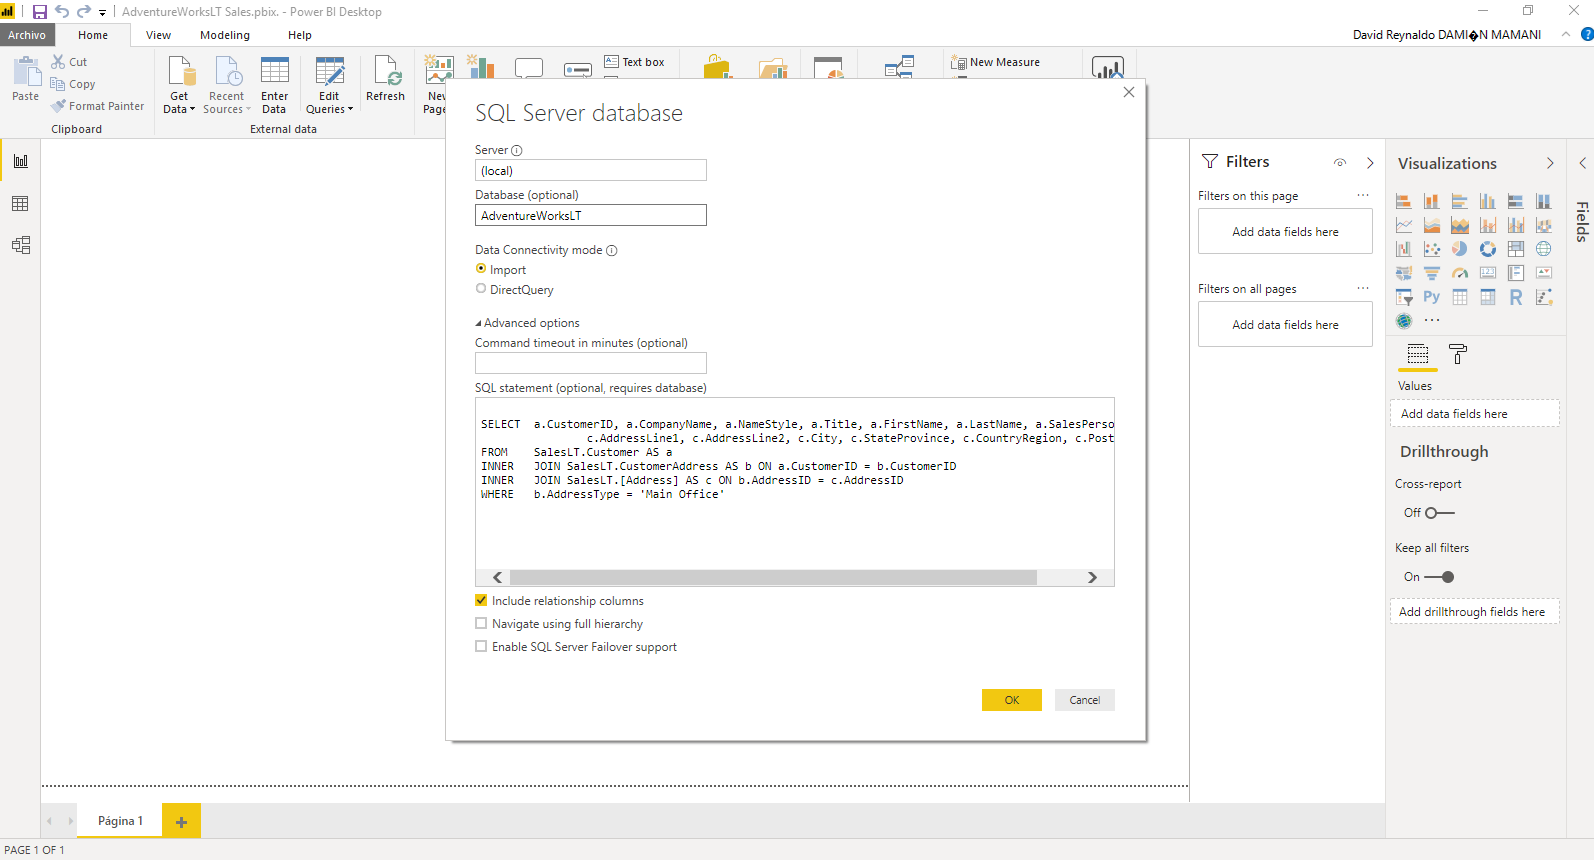
\includegraphics[width=18cm]{./Imagenes/I1}
	\end{center}	
Datos Conectados
\begin{center}
	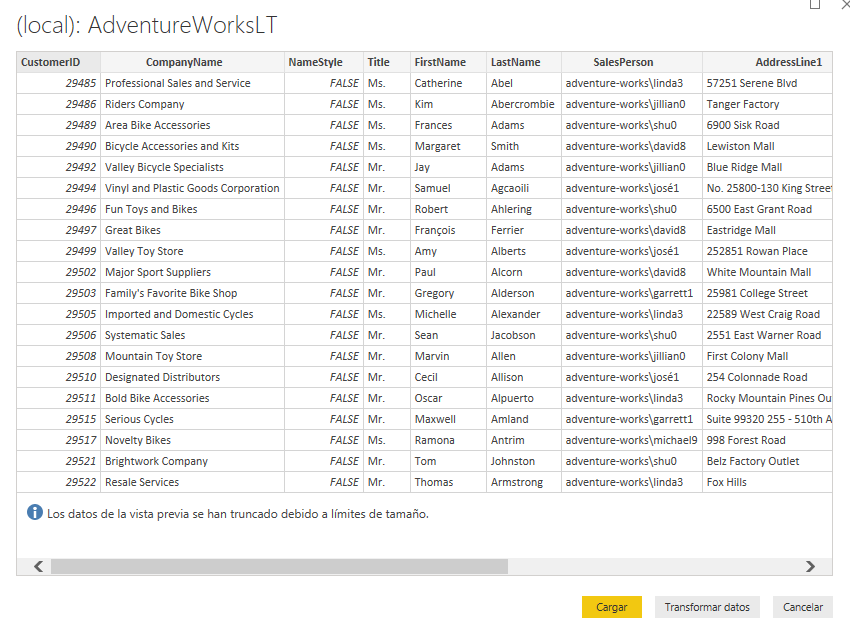
\includegraphics[width=18cm]{./Imagenes/I2}
	\end{center}	

 \item 2.Graficar Datos
Formula cambiada a English (United States). Todos los script insertados de tal manera que nos da los siguientes valores.
	\begin{center}
	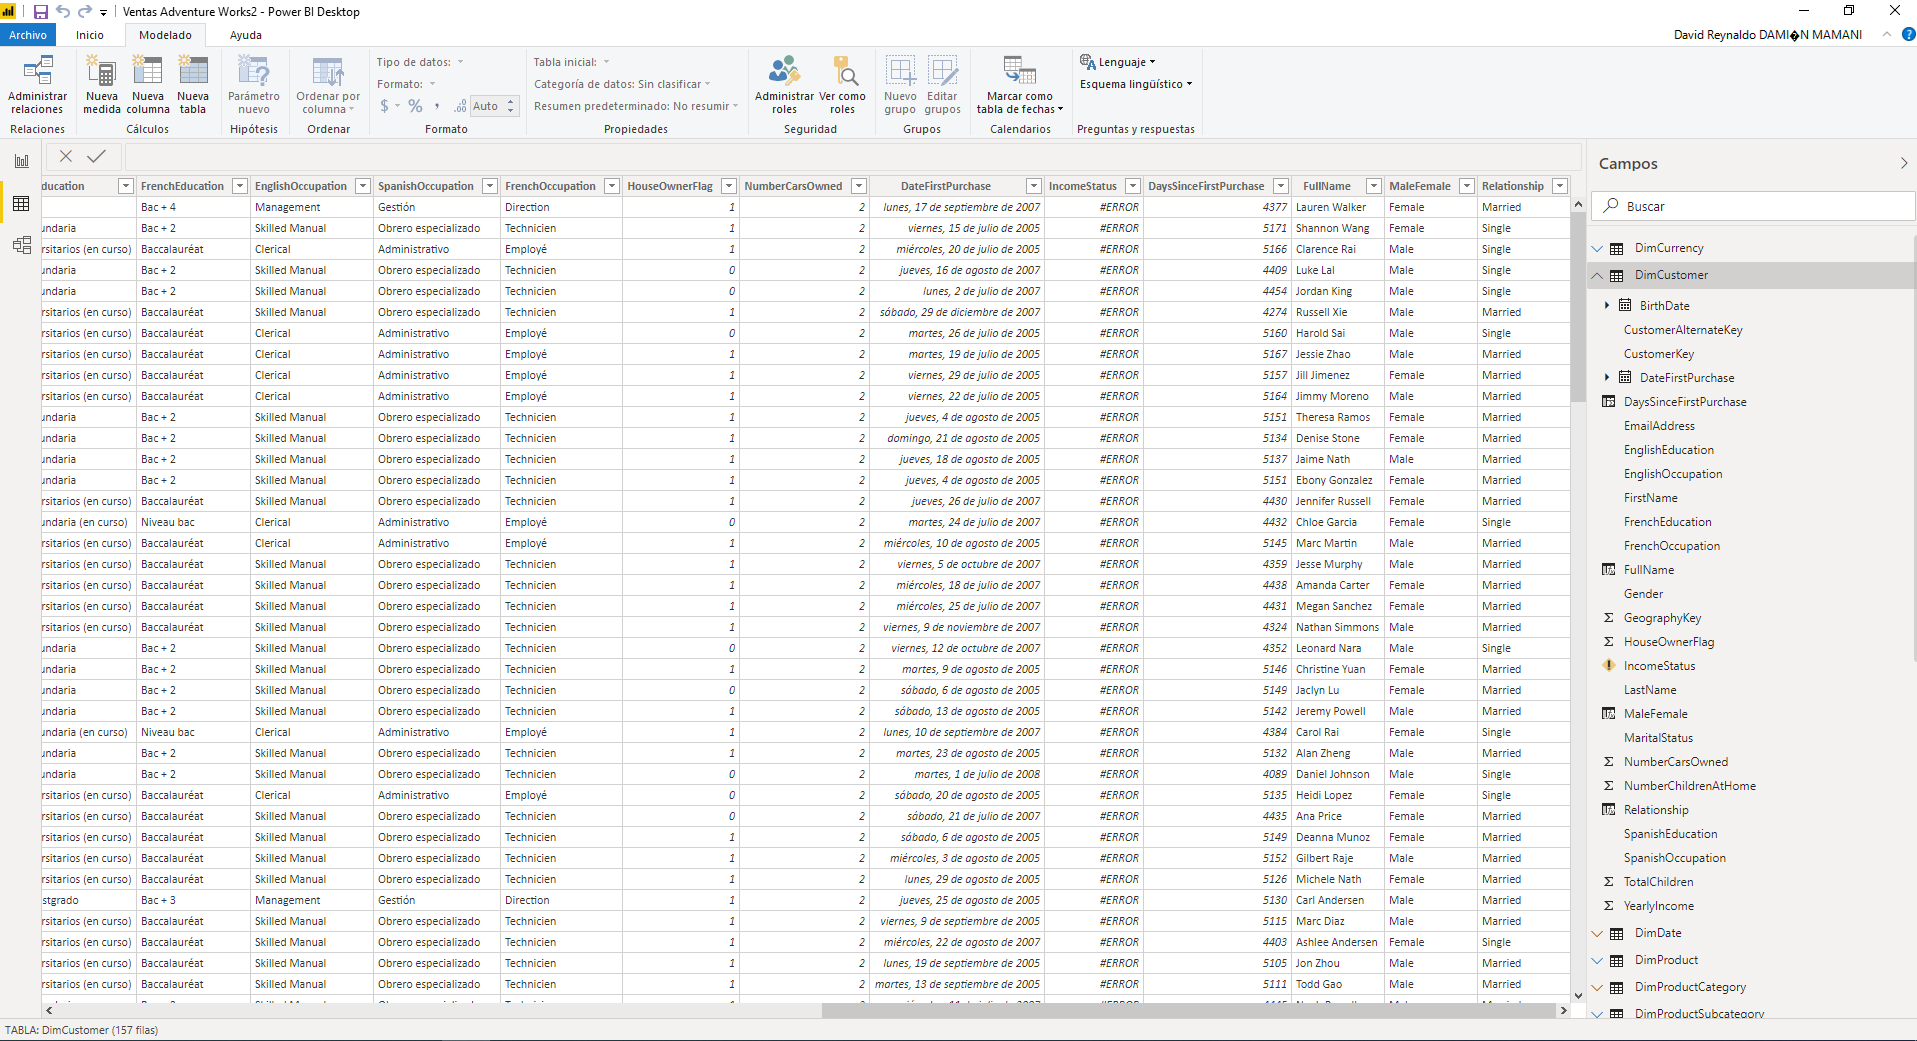
\includegraphics[width=18cm]{./Imagenes/Imagen3}
	\end{center}	

 \item 3.Combinar Data

	\begin{center}
	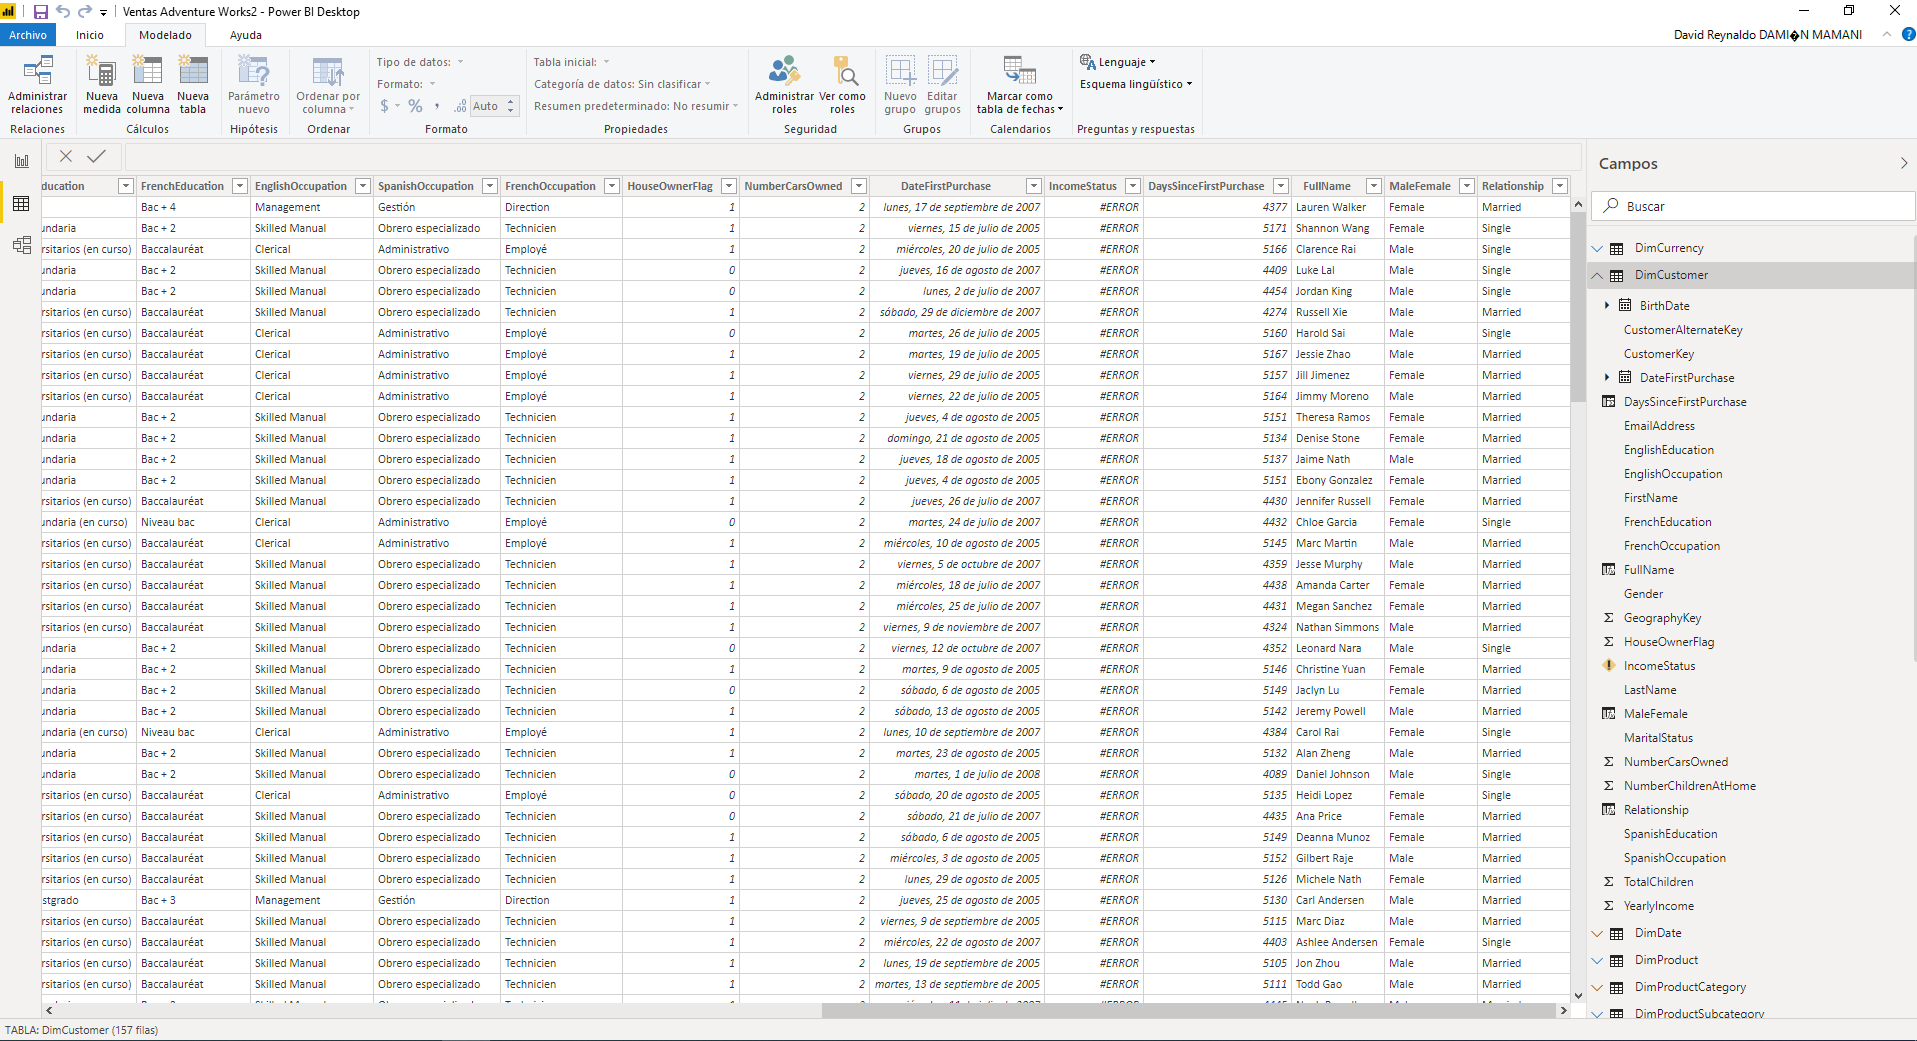
\includegraphics[width=18cm]{./Imagenes/Imagen3}
	\end{center}	
\end{itemize}

\subsection {Construyendo Reportes en Power BI}









\end{document}
